\documentclass[a4paper,10pt]{article}
\usepackage[a4paper, total={6in, 8in}]{geometry}
\setlength\parindent{0pt}
\usepackage[utf8]{inputenc}
\usepackage{graphicx} 
\usepackage{amsmath}
\usepackage{amsfonts}
\usepackage{amssymb}
\usepackage{listings}
\usepackage{ragged2e}
\usepackage{listings}
\usepackage{color}
\usepackage{array}
\usepackage[font=small,labelfont=bf]{caption}
\newcolumntype{P}[1]{>{\centering\arraybackslash}p{#1}}

\setlength{\parskip}{\baselineskip}%
\setlength{\parindent}{0pt}%

\begin{document}
\begin{titlepage}
	\centering
	
\includegraphics[width=.6\textwidth]{liu-logo.png}\par
	\vfill
	{\scshape\Large TDDE01 MACHINE LEARNING\par}
	{\huge\bfseries Lab 3 - Report\par}
	\vspace{0.5cm}
	{\large\itshape Lawrence Thanakumar Rajappa (lawra776)\par}
	\vfill
	{\large \today\par}
\end{titlepage}
\definecolor{dkgreen}{rgb}{0,0.6,0}
\definecolor{gray}{rgb}{0.5,0.5,0.5}
\definecolor{mauve}{rgb}{0.58,0,0.82}

\lstset{frame=tb,
  language=R,
  aboveskip=3mm,
  belowskip=3mm,
  showstringspaces=false,
  columns=flexible,
  basicstyle={\small\ttfamily},
  numbers=none,
  numberstyle=\tiny\color{gray},
  keywordstyle=\color{blue},
  commentstyle=\color{dkgreen},
  stringstyle=\color{mauve},
  breaklines=true,
  breakatwhitespace=true,
  tabsize=3
}
\textbf{\underline{Assignment - 1}} \par
The objective of this assignment is to find the temperature readings between 4 AM to 24 PM in an interval of 2 hours with independent variables
date and  place in Sweden. \par
The following data are provided as input for forecasting the temperature
\begin{itemize}
  \item \textbf{Date} : 2019-12-19
  \item \textbf{place}: \textbf{Longitude} :58.4108, \textbf{Latitude} :15.6214
\end{itemize}
The prediction is done using 3 kernels which are guassian kernels and given below
\begin{itemize}
  \item The first to account for the distance from a station to the point of interest.
  \item The second to account for the distance between the day a temperature measurement was made and the day of interest.
  \item The third to account for the distance between the hour of the day a temperature measurement was made and the hour of interest.
\end{itemize}
3 Smoothing coefficients are selected for the above kernels 
\begin{itemize}
  \item h\_distance = 50000  \# m
  \item h\_date = 7 \# days
  \item h\_time = 3 \# hours
\end{itemize}
\textbf{\underline{Geographical Kernel}} \par
The plot below describe the weights which is provided by the 1\textsuperscript{st} kernel for each of the data points based on the distance between two places \par
\begin{center}
  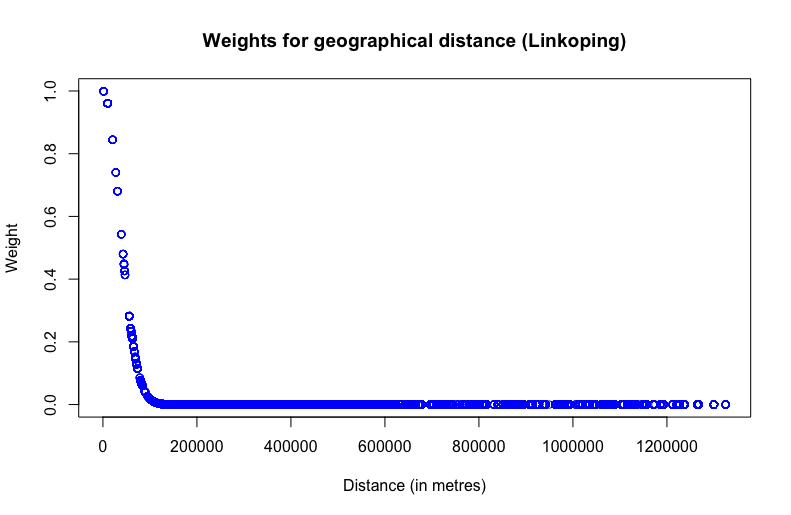
\includegraphics[width=110mm,scale=0.10]{Weights_Distance_1.png}
\end{center}
We can see from the above plot that as we move from the location we want to predict, the weights are getting reduced until they reach 0. This is the expected behaviour,
as one moves away from a location, the temperature calculated becomes irrelavant for the prediction. \par
\textbf{\underline{Day Kernel}} \par
The plot below describe the weights which is provided by the 2\textsuperscript{nd} kernel for each of the data points based on the difference between prediction date and
temperature measured dates (\textit{in days}).
\begin{center}
  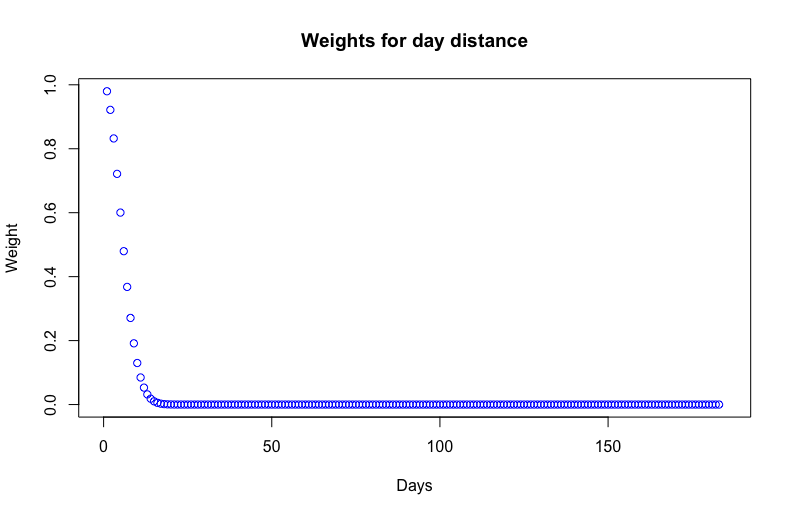
\includegraphics[width=110mm,scale=0.10]{Weights_Day_1.png}
\end{center} 
From the above plot, we could see that as we move away from the date to predict, the weights are getting reduced until they reach 0. This is the expected behaviour,
as one moves away from a day, the temperature measured becomes irrelavant for the prediction\par
\textbf{\underline{Hour Kernel}} \par
The plot below describe the weighs which is provided by the 3\textsuperscript{rd} kernel for each of the data points based on the time difference (\textit{in hours})
\begin{center}
  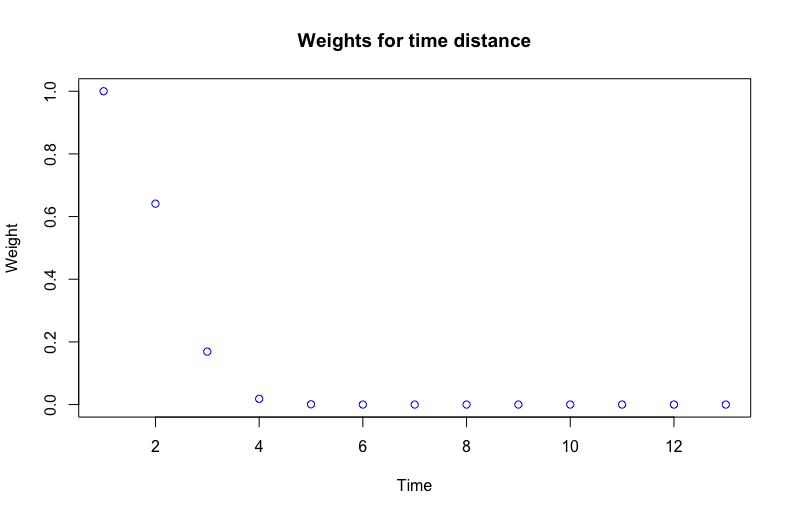
\includegraphics[width=110mm,scale=0.10]{Weights_hour_1.png}
\end{center}
We can see from the above plot that, as we move away from the time we need to predict, the weights are reducing until they reach 0. This is the expected behaviour,
as one moves away from a hour, the temperature measured becomes irrelvant for the prediction.
\newpage
\textbf{\underline{Temperature Prediction for 2019-12-19-Kernel Addition}}
\begin{center}
  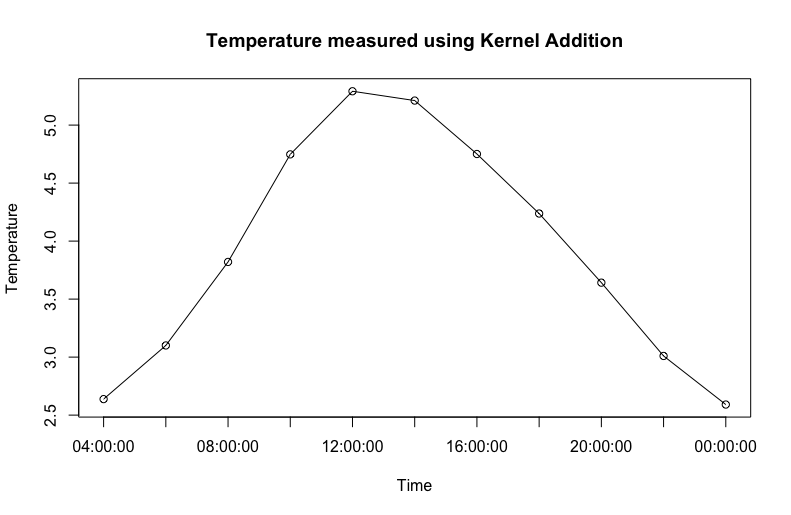
\includegraphics[width=125mm,scale=0.10]{Temp_1_Measured.png}
\end{center}
\textbf{\underline{Temperature Prediction for 2019-12-19-Kernel Multiplication}}
\begin{center}
  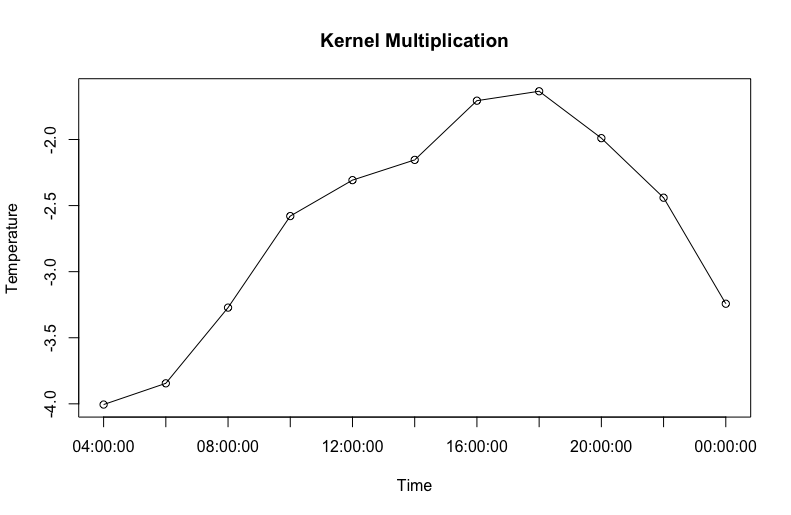
\includegraphics[width=125mm,scale=0.10]{Temp_2_Measured.png}
\end{center}
\newpage
We predict the temperature by using the weighted mean of all observations temperatures. By looking the above two plots,
we can see that multiplied kernel is better than summed kernel, because summed kernel provides higher MSE error rates when
compared with multiplied kernel.\par
\textbf{\underline{Assignment - 3}} \par
In this assignment, we were told to predict values of trignometric function \textit{sin(x)} by using neural network.
This can be achieved by using \textbf{Neuralnet} package in R. \par
Initially, 50 data points (independent variable) are generated randomly between the interval [0,10] and \textit{sin(x)} is applied which is 
dependent variable. The neural network is built with one input node, one hidden layer(10 hidden units of neurons) and 
one output node. \par
Next, weights has to be provided to the neural net in the interval [-1,+1]. So, the 31 (10 biases+10 intercepts for hidden layer) 
and (1 bias + 10 intercepts (from hidden layer) for output node) 31 weights has to be generated. \par
\textbf{\underline{Implementing Neural net}} \par
Before executing neuralnet function, we need to choose optimal threshold. In order to select optimal threshold, we run the 
neural net function for 10 times and calculate the MSE for test data and select the MSE value which is less when compared
with other values and there by selecting the optimal threshold corresponding to that MSE value.

We choose \textbf{4/1000 = 0.004} as the optimal threshold from the plot below which has lower MSE value. The lower MSE value is \textbf{0.0003400358} \par
\begin{center}
  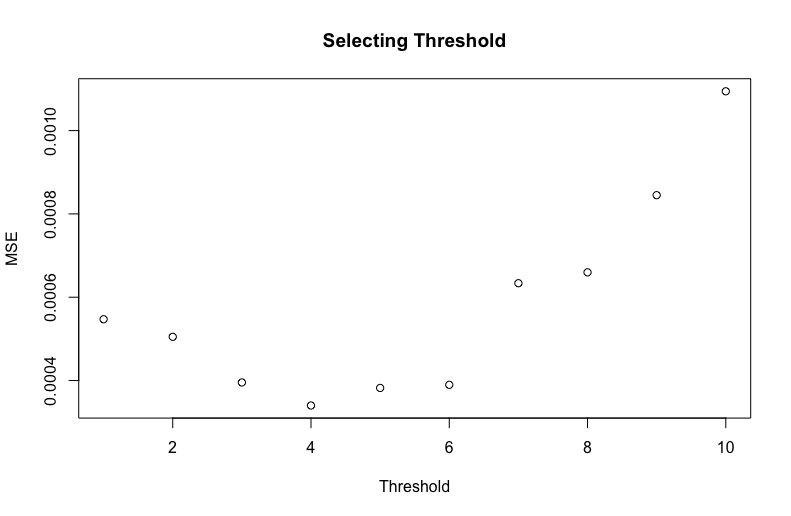
\includegraphics[width=125mm,scale=0.10]{Thresold_plot.png} 
\end{center}
\newpage
Once again, executing the neuralnet function with chosen optimal threshold and below is the result,
\begin{center}
  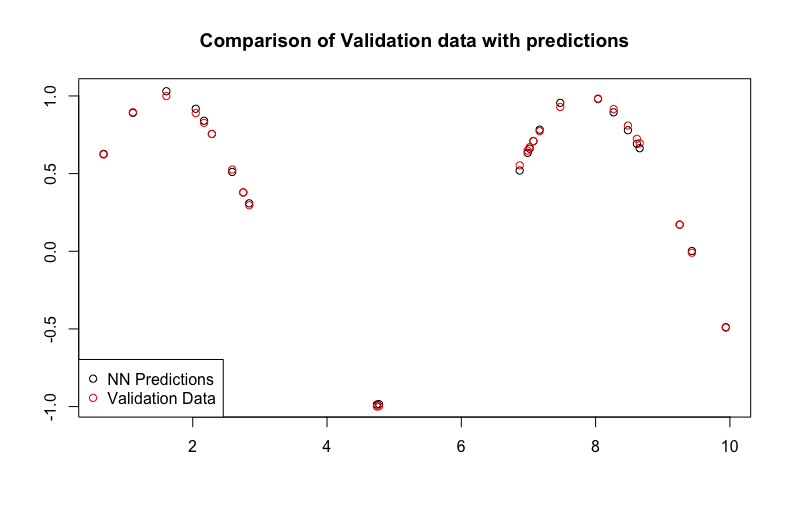
\includegraphics[width=125mm,scale=0.10]{NeuralNet_Predictions.png} 
\end{center}
In order to visualize the network topology with weights and biases, we are plotting the nerual network and it is given below
\begin{center}
  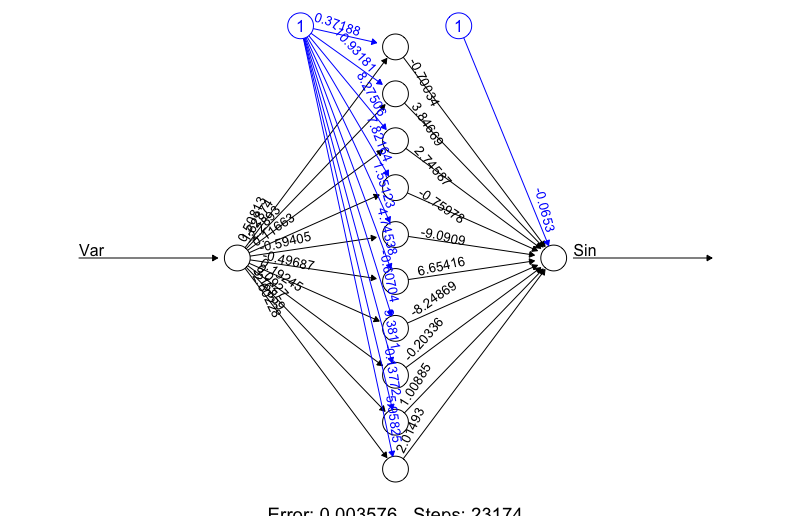
\includegraphics[width=125mm,scale=0.10]{Neural_Net_Topology.png} 
\end{center}
\par
\vspace{0.5cm}
\huge \textbf{\emph{\underline{Code Appendix}}} \par
\large \textit{\textbf{Assignment 1}} \par
\begin{lstlisting}
options(scipen=999) #To avoid scientific notations
RNGversion('3.5.1')

set.seed(1234567890)
library(geosphere)
stations <- read.csv("stations.csv",stringsAsFactors=FALSE, fileEncoding="latin1")
temps <- read.csv("temps50k.csv")
st <- merge(stations,temps,by="station_number")
st$date = as.character(st$date)
st$time = as.character(st$time)

times <- c("04:00:00", "06:00:00","08:00:00","10:00:00","12:00:00","14:00:00", "16:00:00","18:00:00","20:00:00","22:00:00", "00:00:00")
h_distance <- 100000 # These three values are up to the students
h_date <- 7 #days
h_time <- 3 #hours
a <- 58.4108  # The point to predict (up to the students)
b <- 15.6214
latlong = data.frame(latitude = a,longitude = b)
pred_date <- "2019-12-19"
no_of_times = length(times)
latitude = rep(a,no_of_times)
longitude = rep(b,no_of_times)
dates = rep(pred_date,no_of_times)
data_Predict = data.frame(latitude=latitude,longitude=longitude,date=dates,time = times)

colSums(is.na(st))

st = st[as.Date(st$date)<as.Date(pred_date),]

gaussian_Kernel = function(u,h){
  return(exp(-abs(u/h)^2))
}

diff_distance_kernel = function(poi,stations)
{
  distance = distHaversine(poi,stations)
  return(gaussian_Kernel(distance,h_distance))
}

diff_date_kernel = function(doi,day)
{
  day_distance = abs(as.numeric(difftime(strptime(doi,format = "%Y-%m-%d"),strptime(day,format = "%Y-%m-%d"),units = "days")))
  day_distance = day_distance%%365
  day_distance[day_distance>182] = 365-day_distance[day_distance>182]
  return(gaussian_Kernel(day_distance,h_date))
}

diff_hour_kernel = function(hoi,hours)
{
  hour_difference = as.numeric(difftime(as.POSIXct(strptime(hoi, "%H:%M:%S")),
                                        as.POSIXct(strptime(hours, "%H:%M:%S")),
                                        units = "hour"))
  hour_difference = abs(hour_difference)
  hour_difference[hour_difference>12] = 24-hour_difference[hour_difference>12]
  return(gaussian_Kernel(hour_difference,h_time))
}

kernel_calculation_addition = function(toi)
{
  poi_distance = diff_distance_kernel(poi = latlong,stations = st[,4:5])
  doi_distance = diff_date_kernel(pred_date,st$date)
  toi_distance = diff_hour_kernel(toi,st$time)
  
  kernel_Sum = poi_distance + doi_distance + toi_distance
  
  kernel_Sum = (sum(kernel_Sum * st$air_temperature) / sum(kernel_Sum))
 
  return(kernel_Sum)
}

kernel_calculation_multiplication = function(toi)
{
  poi_distance = diff_distance_kernel(poi = latlong,stations = st[,4:5])
  doi_distance = diff_date_kernel(pred_date,st$date)
  toi_distance = diff_hour_kernel(toi,st$time)
  
  kernel_Multiplication = poi_distance * doi_distance * toi_distance
  
  kernel_Multiplication = (sum(kernel_Multiplication * st$air_temperature) / sum(kernel_Multiplication))

  return(kernel_Multiplication)
}

temp_1 = rep(0,length(times))
temp_2 = rep(0,length(times))
i = 0
for(i in 1:length(times)){
  temp_1[i] = kernel_calculation_addition(times[i])
  temp_2[i] = kernel_calculation_multiplication(times[i])
}

plot(temp_1, type="o", xaxt="n", xlab="Time", ylab="Temperature",main="Temperature measured using Kernel Addition")
axis(1, at=1:length(temp_1), labels=times)

plot(temp_2, type="o", xaxt="n", xlab="Time", ylab="Temperature",main="Kernel Multiplication")
axis(1, at=1:length(temp_1), labels=times)

plot(distHaversine(c(a,b),st[4:5]),gaussian_Kernel(distHaversine(c(a,b),st[4:5]),
h_distance),xlab = "Distance",
     ylab = "Weight",main = "Weights for geographical distance",col="blue")
plot(gaussian_Kernel(matrix(seq(1,183,1)),h_date),xlim=c(0,185),xlab="Days",
     ylab="Weight",main = "Weights for day distance",col="blue")
plot(gaussian_Kernel(matrix(seq(0,24,2)),h_time),main="Weights for time distance",
     xlab = "Time",ylab="Weight",col="blue")
\end{lstlisting} \par
\vspace{0.5cm}
\large \textit{\textbf{Assignment 3}} \par
\begin{lstlisting}
  options(scipen=999) #To avoid scientific notations
  RNGversion('3.5.1')
  library(neuralnet)
  library(ggplot2)
  
  set.seed(1234567890)
  Var <- runif(50, 0, 10)
  trva <- data.frame(Var, Sin=sin(Var))
  tr <- trva[1:25,] # Training
  va <- trva[26:50,] # Validation
  ggplot(trva,aes(x=Var,y=Sin))+geom_line()
  # Random initialization of the weights in the interval [-1, 1]
  winit <- runif(31,-1,1)
  #Since we are dealing with regression, best way to choose the model is to use MSE
  mse_test = rep(0,10)
  mse_train = rep(0,10)
  
  for(i in 1:10)
  {
    nn = neuralnet(Sin~Var,data=tr,linear.output = TRUE,threshold = i/1000,hidden = 10,startweights = winit)
    pred = predict(nn,va)
    mse_test[i] = sum((va$Sin-pred)^2)/nrow(va)
    mse_train[i] = sum((tr$Sin-pred)^2)/nrow(tr)
  }
  
  best_Threshold = which(mse_test == min(mse_test))
  plot(1:10,mse_test,xlab="Threshold",ylab = "MSE",main="Selecting Threshold")
  #1st model is having lowest test error when compared with other models.
  nn = neuralnet(Sin~Var,data=tr,linear.output = TRUE,threshold = best_Threshold/1000,hidden = 10,startweights = winit)
  
  plot(prediction(nn)$rep1,col="black",xlab = "",ylab = "")
  points(tr,col="red")
  legend(x="bottomleft",legend = c("NN Predictions","Train Data"),col=c("Black","Red"),pch = c(1,1))
  
  plot(va$Var,predict(nn,va)[,1],col="black",xlab = "",ylab = "",main="Comparison of Validation data with predictions")
  points(va,col="red")
  legend(x="bottomleft",legend = c("NN Predictions","Validation Data"),col=c("Black","Red"),pch = c(1,1))
  
  plot(nn,rep="best")  
\end{lstlisting}
\end{document}